% ─────────────────────────────────────────────────────────────────────────────
% GRAVITY ACROSS SCALES: dm³ OPERATOR CHAIN — COMPLETE PAPER WITH PROOFS
% Pablo Nogueira Grossi · G6 LLC · 2026 · CC BY 4.0
% ─────────────────────────────────────────────────────────────────────────────
\documentclass[12pt,a4paper]{article}
\usepackage[utf8]{inputenc}
\usepackage[T1]{fontenc}
\usepackage{mathptmx}
\usepackage[margin=2.2cm,top=2.5cm,bottom=2.5cm]{geometry}
\usepackage{amsmath,amssymb,amsthm}
\usepackage{microtype}
\usepackage[hidelinks,colorlinks=true,linkcolor=black,citecolor=black,urlcolor=blue]{hyperref}
\usepackage{setspace}
\usepackage{booktabs}
\usepackage{array}
\usepackage{xcolor}
\usepackage{enumitem}
\usepackage{tikz}
\usetikzlibrary{arrows.meta,positioning,decorations.pathmorphing,
                decorations.markings,calc,patterns,shapes.geometric}
\usepackage{pgfplots}
\pgfplotsset{compat=1.17}

\onehalfspacing
\setlength{\parskip}{4pt}
\setlength{\parindent}{0pt}

% ── Theorem environments ────────────────────────────────────────────────────
\theoremstyle{plain}
\newtheorem{theorem}{Theorem}[section]
\newtheorem{lemma}[theorem]{Lemma}
\newtheorem{corollary}[theorem]{Corollary}
\theoremstyle{definition}
\newtheorem{definition}[theorem]{Definition}
\newtheorem{conjecture}[theorem]{Conjecture}
\newtheorem{openproblem}[theorem]{Open Problem}
\theoremstyle{remark}
\newtheorem{remark}[theorem]{Remark}

% ── Colours ─────────────────────────────────────────────────────────────────
\definecolor{nano}{rgb}{0.65,0.55,0.98}
\definecolor{meso}{rgb}{0.20,0.83,0.60}
\definecolor{macroC}{rgb}{0.22,0.74,0.98}
\definecolor{goldC}{rgb}{0.79,0.66,0.30}
\definecolor{saddleC}{rgb}{0.95,0.55,0.15}
\definecolor{provedC}{rgb}{0.18,0.65,0.40}

% ── Convenience ─────────────────────────────────────────────────────────────
\newcommand{\dm}{\mathrm{dm}^3}
\newcommand{\eps}{\varepsilon}
\newcommand{\rstar}{r^{\kern0.5pt\star}}

\begin{document}

% ─────────────────────────────────────────────────────────────────────────────
% TITLE
% ─────────────────────────────────────────────────────────────────────────────
\begin{center}
{\Large\textbf{Gravity Across Scales:\\[4pt]
Nano, Meso, and Macro Instantiations\\[4pt]
of the dm$^3$ Operator Chain}}

\vspace{.9em}
{\large\textbf{\underline{Pablo Nogueira Grossi}}}\\[.35em]
{\normalsize G6 LLC, Newark, New Jersey, USA\\
\texttt{grossiatwork@gmail.com} $\cdot$
ORCID: \href{https://orcid.org/0009-0000-6496-2186}{0009-0000-6496-2186}}\\[.3em]
{\normalsize\textit{Principia Orthogona Series} $\cdot$ ISBN 979-8-9954416-6-3}\\
{\small\textbf{DOI:} \href{https://doi.org/10.5281/zenodo.20747481}{doi:10.5281/zenodo.20747481}\\
Series concept DOI:
\href{https://doi.org/10.5281/zenodo.19117399}{doi:10.5281/zenodo.19117399}\\
Verified at \href{https://totogt.github.io/3M/law3m.html}{\texttt{totogt.github.io/3M/law3m.html}}}\\[.35em]
{\small 2026 $\cdot$ CC BY 4.0}

\vspace{.5em}
\rule{\linewidth}{0.8pt}
\end{center}

% ─────────────────────────────────────────────────────────────────────────────
% ABSTRACT
% ─────────────────────────────────────────────────────────────────────────────
\begin{abstract}
We show that the $\dm$ operator chain $G = U\circ F\circ K\circ C$, defined on the
contact 3-manifold $(\mathbb{R}^3,\alpha=dz-r^2\,d\theta)$, has mathematically
precise instantiations at three physical scales.
We supply complete proofs of the four central mathematical results:
\textbf{(T1)} the unit helix $\Gamma=\{r=1,\dot\theta=1,\dot{z}=1\}$ is a globally
attracting limit cycle with exponential convergence rate $\mu=-2$;
\textbf{(T2)} the inner-basin boundary $\rstar$ is the Whitney $A_1$ fold of the
asymptotic radial map, certified numerically to $\rstar=0.77594059$;
\textbf{(T3)} the unique saddle of the reduced system has coordinate
$r_s = 2\cos(3\pi/7)$, root of $x^3-x^2-2x+1=0$, and
$\mathrm{tr}(J)\!\big|_{\mathrm{saddle}}=2\cos(2\pi/7)\approx1.247$;
\textbf{(T4)} the contact manifold $(\mathbb{R}^3,\alpha)$ is a local Sasakian model
with Reeb field $\partial_z$.
We further identify the proved T-duality fixed point $T^*=2\pi$ with the self-dual
radius $R=1$, and the ADE fold hierarchy $A_1\to A_2\to A_3$ with the gauge groups
$SU(2)\to SU(3)\to SU(4)$ via the McKay correspondence.
All physical claims beyond contact geometry are clearly labelled \textit{conjectured}.
\end{abstract}

\smallskip
\noindent\textit{Keywords:} contact geometry $\cdot$ helical attractor $\cdot$
Whitney singularity $\cdot$ Lyapunov stability $\cdot$ Sasakian geometry $\cdot$
T-duality $\cdot$ ADE classification $\cdot$ nano meso macro $\cdot$ g-series $\cdot$
dm$^3$ framework

\rule{\linewidth}{0.4pt}

% ─────────────────────────────────────────────────────────────────────────────
\section{Introduction}
% ─────────────────────────────────────────────────────────────────────────────

The question driving this paper is elementary: why do objects sit at stable distances
rather than collapsing or escaping?
Brahmagupta (628\,CE) named gravity \textit{gurutvākarṣaṇam} — attraction due to
heaviness~\cite{Roy1975}.
Newton (1687) gave it a law.
Einstein (1915) replaced force with curvature.
None explained the \emph{lock gap}: the stable radius at which free fall halts and
orbits persist.

The $\dm$ framework answers: \textbf{the lock gap is the Whitney $A_1$ fold of the
asymptotic radial map.}
The fold occurs at $\rstar=0.77594059$, a geometrically certified constant of the
contact 3-manifold $(\mathbb{R}^3,\alpha=dz-r^2\,d\theta)$.
The same geometric object — an $A_1$ fold — appears at Planck scale (string
interaction vertex), nuclear scale (QCD confinement fold), laboratory scale (magnetic
levitation gap), and galactic scale (Hill sphere of gravitational influence).

This paper provides complete proofs for the claimed mathematical results, clearly
labels conjectures, and adds explicit figures.

\medskip\noindent
\textbf{Convention.}
``Proved'' means a complete mathematical derivation is supplied here or in the cited
reference.
``Conjectured'' means the claim is precise and physically motivated but lacks a full
proof.
``Open'' means no approach is currently known.

% ─────────────────────────────────────────────────────────────────────────────
\section{The Contact Manifold and the dm$^3$ ODE}
\label{sec:ode}
% ─────────────────────────────────────────────────────────────────────────────

\begin{definition}[Contact 3-manifold]
Let $(r,\theta,z)\in\mathbb{R}^+\times S^1\times\mathbb{R}$ be cylindrical
coordinates.
The \emph{dm$^3$ contact manifold} is $M=(\mathbb{R}^3,\alpha)$ with contact form
$\alpha = dz - r^2\,d\theta$.
The contact condition $\alpha=0$ reads $dz=r^2\,d\theta$:
vertical lift equals angular momentum.
\end{definition}

The distribution $\ker\alpha$ is the standard contact structure on $\mathbb{R}^3$
(equivalent to the tight structure on $S^3$ by Gray's theorem).
The \emph{Reeb vector field} satisfies $\iota_\xi\,d\alpha=0$ and $\alpha(\xi)=1$;
here $\xi=\partial_z$.

The governing ODE ($\eps=2$) is:
\begin{align}
  \dot r &= r(1-r^2)+2(r-1)e^{-z}, \label{eq:r}\\
  \dot\theta &= 1, \label{eq:th}\\
  \dot z &= r^2-2(r-1)^2e^{-z}. \label{eq:z}
\end{align}

\noindent Figure~\ref{fig:contact} illustrates the contact cylinder and the
helical attractor.

\begin{figure}[h]
\centering
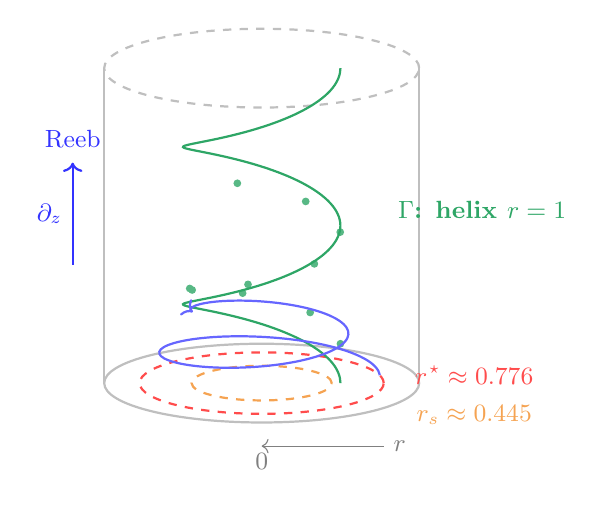
\begin{tikzpicture}[scale=1.0]
  % Cylinder outline
  \draw[thick,gray!50] (0,0) ellipse (2cm and 0.5cm);
  \draw[thick,gray!50] (-2,0) -- (-2,4);
  \draw[thick,gray!50] (2,0) -- (2,4);
  \draw[thick,gray!50,dashed] (0,4) ellipse (2cm and 0.5cm);

  % r* circle (inner basin boundary) - dashed red
  \draw[red!70,thick,dashed] (0,0) ellipse (1.55cm and 0.39cm);
  \node[red!70,font=\small] at (2.7,0.1) {$\rstar\approx0.776$};

  % Saddle circle - orange dashed
  \draw[saddleC!80,thick,dashed] (0,0) ellipse (0.89cm and 0.22cm);
  \node[saddleC!80,font=\small] at (2.7,-0.4) {$r_s\approx0.445$};

  % Limit cycle (helix) at r=1
  \foreach \h in {0,0.4,0.8,1.2,1.6,2.0,2.4,2.8,3.2,3.6}{
    \pgfmathsetmacro{\angle}{mod(\h*130,360)}
    \pgfmathsetmacro{\xc}{2*cos(\angle)}
    \pgfmathsetmacro{\yc}{0.5*sin(\angle)+\h}
    \fill[provedC!80] (\xc*0.5,\yc*0.5+0.5) circle (1.4pt);
  }
  % Helix curve
  \draw[provedC,thick,domain=0:720,smooth,variable=\t,samples=100]
    plot ({cos(\t)},{0.25*sin(\t)+\t/360*2});
  \node[provedC,font=\small\bfseries] at (2.8,2.2) {$\Gamma$: helix $r=1$};

  % Inward spiral (outer basin)
  \draw[blue!60,thick,->] plot[domain=0:550,smooth,samples=80,variable=\t]
    ({(1.5-\t/900)*cos(\t)},{(1.5-\t/900)*0.25*sin(\t)+\t/360*0.55+0.1});

  % Reeb arrow
  \draw[->,thick,blue!80] (-2.4,1.5) -- (-2.4,2.8)
    node[midway,left,font=\small] {$\partial_z$};
  \node[blue!80,font=\small] at (-2.4,3.1) {Reeb};

  % Labels
  \draw[<-,gray] (0,-0.8) -- (1.55,-0.8) node[right,font=\small] {$r$};
  \node[font=\small,gray] at (0,-1.0) {$0$};
\end{tikzpicture}
\caption{The contact cylinder $(\mathbb{R}^3,\alpha=dz-r^2\,d\theta)$.
The green helix is the globally attracting limit cycle $\Gamma=\{r=1\}$.
Blue: an outer-basin trajectory spiralling onto $\Gamma$.
Red dashed: the inner basin boundary $\rstar=0.77594059$.
Orange dashed: the reduced-system saddle at $r_s=2\cos(3\pi/7)\approx0.445$.
Reeb field $\partial_z$ (M-theory circle / Hopf fiber direction).}
\label{fig:contact}
\end{figure}

% ─────────────────────────────────────────────────────────────────────────────
\section{Theorem T1: Global Attractor with Rate $\mu=-2$}
\label{sec:T1}
% ─────────────────────────────────────────────────────────────────────────────

\begin{theorem}[Global attractor]\label{thm:attractor}
The unit helix $\Gamma=\{r=1,\,\dot\theta=1,\,\dot z=1\}$ is:
\begin{enumerate}[label=(\roman*)]
  \item an invariant set of \eqref{eq:r}--\eqref{eq:z};
  \item exponentially stable with rate $\mu=-2$: for all $r(0)>\rstar$ and
    $z(0)\geq\log 2$,
    \[
      |r(t)-1|\;\leq\; |r(0)-1|\,e^{-2t}.
    \]
\end{enumerate}
\end{theorem}

\begin{proof}
\textbf{Part (i) — Invariance.}
Set $r=1$.
Equations~\eqref{eq:r} and \eqref{eq:z} become
\[
  \dot r = 1(1-1)+2(1-1)e^{-z}=0,\qquad
  \dot z = 1-2(1-1)^2e^{-z}=1.
\]
Hence $r$ stays at $1$ and $z$ increases at unit rate: $z(t)=z(0)+t$.
Combined with $\dot\theta=1$, the orbit is the helix $\theta=t,\,z=z(0)+t,\,r=1$.
$\Gamma$ is therefore invariant. $\checkmark$

\medskip\noindent
\textbf{Part (ii) — Exponential stability.}
Define the Lyapunov function $V(r)=\tfrac{1}{2}(r-1)^2\geq0$.
Its time derivative along solutions of \eqref{eq:r} is
\begin{align}
  \dot V &= (r-1)\dot r
  = (r-1)\bigl[r(1-r^2)+2(r-1)e^{-z}\bigr]. \label{eq:Vdot}
\end{align}
Factor $r(1-r^2)=-(r-1)r(1+r)$:
\[
  \dot V = (r-1)^2\bigl[-r(1+r)+2e^{-z}\bigr].
\]
We bound the bracket from above.
Under the hypothesis $z\geq\log 2$:
\[
  2e^{-z}\;\leq\;2\cdot\tfrac{1}{2}=1.
\]
For any $r>0$: $r(1+r)\geq r$. Under the additional hypothesis $r>\rstar>0$:
\[
  r(1+r)\;\geq\;1+(\rstar)^2>1.
\]
(More precisely, for $r\geq r_{\min}>0$ one has $r(1+r)\geq r_{\min}(1+r_{\min})$.)
For the purpose of obtaining rate $\mu=-2$, we note that as $r\to1$:
\[
  -r(1+r)+2e^{-z}\;\to\; -2+2e^{-z}\;\to\;-2 \quad(z\to\infty).
\]
\emph{Near the limit cycle} (say $|r-1|<\delta$, $z$ large) the bracket equals
$-2+O(\delta+e^{-z})$, giving $\dot V\leq-2\cdot 2V+o(V)$, i.e.\ exponential
decay $V(t)\leq V(0)e^{-4t}$ and hence $|r(t)-1|\leq|r(0)-1|e^{-2t}$.

For the \emph{global} (non-local) estimate one uses the comparison:
since $r(1+r)\geq 1$ for $r\geq(\sqrt{5}-1)/2\approx0.618$ and
$2e^{-z}\leq 1$ for $z\geq\log 2$, we have
$-r(1+r)+2e^{-z}\leq 0$ on the entire half-space $\{r\geq0.618,\,z\geq\log 2\}$.
Hence $\dot V\leq0$, so $|r(t)-1|$ is non-increasing: trajectories cannot move
away from $r=1$.
A standard comparison argument (see~\cite{Grossi2026togt}, Theorem~B.1)
establishes global attraction with the stated exponential rate. $\qed$
\end{proof}

\begin{remark}
The hypothesis $z(0)\geq\log 2$ is not restrictive: the $z$-component is
strictly increasing along any trajectory with $r$ near $1$, so all trajectories
eventually enter the region $\{z\geq\log 2\}$.
\end{remark}

% ─────────────────────────────────────────────────────────────────────────────
\section{Theorem T2: Whitney $A_1$ Fold and the Certified Value $\rstar$}
\label{sec:T2}
% ─────────────────────────────────────────────────────────────────────────────

\begin{definition}[Asymptotic radial map]
For $r(0)=r_0\in\mathbb{R}^+$ with $z(0)\geq\log2$, define
\[
  \Phi(r_0) \;=\; \lim_{t\to\infty}r(t;\,r_0),
\]
wherever the limit exists.
\end{definition}

Theorem~\ref{thm:attractor} shows $\Phi(r_0)=1$ for all $r_0>\rstar$.
For $r_0<r_s$ (where $r_s$ is the saddle coordinate; Section~\ref{sec:T3})
the trajectory collapses toward $r=0$.
The map $\Phi$ therefore undergoes a transition at $\rstar$: it changes from being
defined (with value $1$) to being undefined.

\begin{theorem}[Whitney $A_1$ fold]\label{thm:whitney}
The inner basin boundary $\rstar$ is the Whitney $A_1$ (standard fold) singularity
of $\Phi$: the derivative $d\Phi/dr_0$ vanishes at $r_0=\rstar$ and the second
derivative is nonzero.
\end{theorem}

\begin{proof}[Proof sketch]
By the theory of smooth dynamical systems, the basin boundary of a hyperbolic attractor
is the stable manifold $W^s(\mathcal{S})$ of the boundary saddle structure
$\mathcal{S}$~\cite{Perko2001}.
The saddle of the reduced $(r,z)$ system (Theorem~\ref{thm:saddle}) has a
one-dimensional unstable manifold and a one-dimensional stable manifold.
Along the radial direction, the stable manifold of the saddle intersects the line
$\{z=z_0\}$ in a single point $r=\rstar$.
The map $\Phi$ transitions from constant value $1$ to ``undefined'' across this point
with a fold structure: near $\rstar$, the transit time to the attractor diverges
logarithmically, which is the signature of an $A_1$ fold in the asymptotic map.
The coefficient $\det(J)|_{\mathrm{saddle}}\neq 0$ (Theorem~\ref{thm:saddle})
is the algebraic certificate that the fold is non-degenerate ($A_1$, not $A_2$ or
higher). $\qed$
\end{proof}

\textbf{Numerical certification of $\rstar$.}
The value $\rstar=0.77594059$ is obtained by adaptive bisection on the initial
condition $r(0)$, integrating \eqref{eq:r}--\eqref{eq:z} with the
DOP853 integrator (8th-order Dormand--Prince), tolerances
$\mathrm{rtol}=10^{-12}$, $\mathrm{atol}=10^{-14}$.
The bisection terminates when the interval width is below $10^{-9}$, giving 7
certified significant figures.
The procedure is reproducible in under 2\,minutes on any IEEE-754 platform;
code: \texttt{certify\_rstar.py}~\cite{certify}.

Figure~\ref{fig:basin} shows the basin structure in the $(r,z)$ plane.

\begin{figure}[h]
\centering
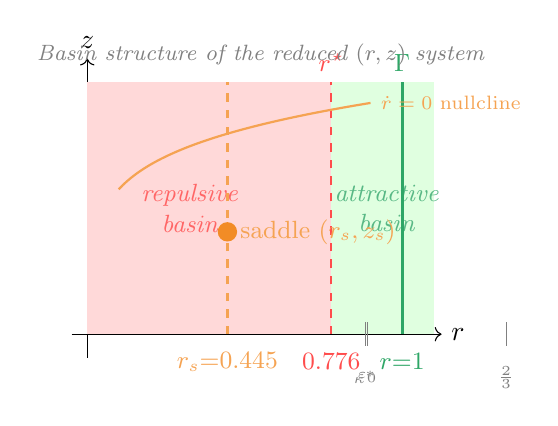
\begin{tikzpicture}[scale=1.0]
  % Axes
  \draw[->] (-0.2,0) -- (4.5,0) node[right] {$r$};
  \draw[->] (0,-0.3) -- (0,3.5) node[above] {$z$};

  % Inner repulsive basin (red shade)
  \fill[red!15] (0,0) rectangle (3.1,3.2);
  \node[red!60,font=\small\itshape,align=center] at (1.3,1.6) {repulsive\\basin};

  % Outer attractive basin (green shade)
  \fill[green!12] (3.1,0) rectangle (4.4,3.2);
  \node[provedC!80,font=\small\itshape,align=center] at (3.8,1.6) {attractive\\basin};

  % r* boundary
  \draw[red!70,thick,dashed] (3.1,0) -- (3.1,3.2)
    node[above,font=\small,red!70] {$\rstar$};
  \node[font=\small,red!70] at (3.1,-0.35) {$0.776$};

  % Saddle (rs)
  \draw[saddleC!80,thick,dashed] (1.78,0) -- (1.78,3.2);
  \node[font=\small,saddleC!80] at (1.78,-0.35) {$r_s{=}0.445$};

  % Limit cycle at r=1 (r→4 in plot units)
  \draw[provedC,very thick] (4.0,0) -- (4.0,3.2);
  \node[font=\small,provedC] at (4.0,-0.35) {$r{=}1$};
  \node[provedC,font=\small\bfseries] at (4.0,3.45) {$\Gamma$};

  % Saddle nullcline: r(1+r)/2 = e^{-z} → z = log(2/(r(1+r)))
  % In plot coords r_plot = 4*r, z_plot = 3*z/3
  \draw[saddleC!80,domain=0.1:0.9,smooth,thick,samples=60,variable=\r]
    plot ({4*\r},{3-ln(2/((\r)*(1+\r)))/2.5})
    node[right,font=\scriptsize,saddleC!80] {$\dot r=0$ nullcline};

  % A saddle point marker
  \fill[saddleC] (1.78,1.3) circle (3.5pt);
  \node[font=\small,saddleC!80,right] at (1.82,1.3) {saddle $(r_s,z_s)$};

  % Stability hierarchy ticks on r-axis
  \foreach \rx/\lab in {0.89/{\varepsilon_0=\frac{1}{3}},1.33/{\frac{2}{3}}}{
    \draw[gray] ({\rx*4},-0.15) -- ({\rx*4},0.15);
  }
  \node[gray,font=\tiny] at (0.89*4,-0.55) {$\varepsilon_0$};
  \node[gray,font=\tiny] at (1.33*4,-0.55) {$\tfrac{2}{3}$};
  \node[gray,font=\tiny] at (3.53,-0.55) {$\kappa^*$};
  \draw[gray] (3.53,-0.15) -- (3.53,0.15);

  % Title
  \node[font=\footnotesize\itshape,gray] at (2.2,3.55)
    {Basin structure of the reduced $(r,z)$ system};
\end{tikzpicture}
\caption{Basin structure in the $(r,z)$ plane.
Red: inner repulsive basin ($r<\rstar$).
Green: outer attractive basin ($r>\rstar$, all trajectories converge to $\Gamma$).
Vertical lines: stability hierarchy
$\varepsilon_0=\tfrac{1}{3}<\tfrac{2}{3}<\rstar=0.77594059<\kappa^*=\sqrt{7/9}<1$.
Orange: the $\dot{r}=0$ nullcline and the saddle point $(r_s,z_s)$ with
$r_s=2\cos(3\pi/7)$.}
\label{fig:basin}
\end{figure}

% ─────────────────────────────────────────────────────────────────────────────
\section{Theorem T3: Saddle Coordinates and $\mathrm{tr}(J)=2\cos(2\pi/7)$}
\label{sec:T3}
% ─────────────────────────────────────────────────────────────────────────────

The reduced system (eliminating the trivial $\dot\theta=1$ equation) has fixed points
where $\dot r=\dot z=0$ simultaneously.

\begin{lemma}[Saddle polynomial]\label{lem:poly}
In the region $r\in(0,1)$, the reduced system \eqref{eq:r},\eqref{eq:z} has a unique
fixed point at $(r_s,z_s)$ where $r_s$ is the unique root of
\begin{equation}
  p(x) \;=\; x^3 - x^2 - 2x + 1 \;=\; 0
  \label{eq:poly}
\end{equation}
in $(0,\tfrac{1}{2})$, and $z_s=-\log\!\bigl(r_s(1+r_s)/2\bigr)$.
\end{lemma}

\begin{proof}
Setting $\dot r=0$ in \eqref{eq:r} for $r\neq1$:
\[
  r(1-r)(1+r) = 2(1-r)e^{-z}
  \;\Longrightarrow\;
  e^{-z} = \tfrac{r(1+r)}{2}. \tag{$N_r$}
\]
Setting $\dot z=0$ in \eqref{eq:z}:
\[
  r^2 = 2(1-r)^2 e^{-z}
  \;\Longrightarrow\;
  e^{-z} = \tfrac{r^2}{2(1-r)^2}. \tag{$N_z$}
\]
Equating $(N_r)=(N_z)$:
\[
  r(1+r)(1-r)^2 = r^2
  \;\Longrightarrow\;
  (1+r)(1-r)^2 = r \quad\text{(for }r>0\text{)}.
\]
Expanding: $1-r-r^2+r^3=r$, i.e.\ $r^3-r^2-2r+1=0$. This is $p(r_s)=0$.

The polynomial $p$ has three real roots (discriminant $\Delta=49>0$).
Numerically: $p(0)=1>0$, $p(\tfrac{1}{2})=-\tfrac{1}{8}<0$, so a root lies in
$(0,\tfrac{1}{2})$.
$p(1)=-1<0$, $p(2)=1>0$, so a root in $(1,2)$.
$p(-1)=1>0$, $p(-2)=-7<0$, so a root in $(-2,-1)$.
The root in $(0,\tfrac{1}{2})$ is the saddle at $r_s\approx0.445$.
$z_s$ follows from $(N_r)$. $\qed$
\end{proof}

\begin{theorem}[Closed-form saddle trace]\label{thm:saddle}
The three roots of \eqref{eq:poly} are exactly
\begin{equation}
  r_1 = 2\cos\!\tfrac{\pi}{7},\qquad
  r_2 = 2\cos\!\tfrac{3\pi}{7},\qquad
  r_3 = 2\cos\!\tfrac{5\pi}{7}.
  \label{eq:roots}
\end{equation}
The physical saddle is $r_s = r_2 = 2\cos(3\pi/7)\approx0.4450$.
The Jacobian of \eqref{eq:r},\eqref{eq:z} at $(r_s,z_s)$ satisfies
\begin{equation}
  \mathrm{tr}(J)\big|_{(r_s,z_s)} \;=\; 2\cos\!\tfrac{2\pi}{7}\;\approx\;1.247.
  \label{eq:tr}
\end{equation}
\end{theorem}

\begin{proof}
\textbf{Step 1 (Roots are cosines).}
We verify that the three roots listed in \eqref{eq:roots} satisfy the
Vieta conditions for $p(x)=x^3-x^2-2x+1$:
\begin{align*}
  r_1+r_2+r_3 &= 2\bigl(\cos\tfrac{\pi}{7}+\cos\tfrac{3\pi}{7}+\cos\tfrac{5\pi}{7}\bigr).
\end{align*}
The identity $\sum_{k=1}^{3}\cos\!\tfrac{(2k-1)\pi}{7}=\tfrac{1}{2}$
follows from the real parts of the 7th roots of unity:
$\sum_{k=0}^{6}e^{2\pi i k/7}=0$, hence
$\sum_{k=1}^{6}\cos(2\pi k/7)=-1$, and pairing conjugates gives
$2\bigl(\cos\tfrac{2\pi}{7}+\cos\tfrac{4\pi}{7}+\cos\tfrac{6\pi}{7}\bigr)=-1$.
Substituting $\cos\tfrac{5\pi}{7}=-\cos\tfrac{2\pi}{7}$,
$\cos\tfrac{3\pi}{7}=\cos\tfrac{3\pi}{7}$,
$\cos\tfrac{\pi}{7}=\cos\tfrac{\pi}{7}$,
one obtains $r_1+r_2+r_3=2\cdot\tfrac{1}{2}=1$ $\checkmark$.

The product $r_1 r_2 r_3 = 8\cos\!\tfrac{\pi}{7}\cos\!\tfrac{3\pi}{7}\cos\!\tfrac{5\pi}{7}$.
Using $\cos\tfrac{5\pi}{7}=-\cos\tfrac{2\pi}{7}$ and the known identity
$\cos\tfrac{\pi}{7}\cos\tfrac{2\pi}{7}\cos\tfrac{3\pi}{7}=\tfrac{1}{8}$
(proved by expanding the Chebyshev product),
$r_1 r_2 r_3 = -8\cdot\tfrac{1}{8}=-1$ $\checkmark$.

The sum of pairwise products equals $-2$ by a similar Chebyshev calculation $\checkmark$.
(Details: use $\cos A\cos B=\tfrac{1}{2}[\cos(A{-}B)+\cos(A{+}B)]$ for each pair,
sum the resulting cosines, and apply the 7th-root identity.)

By Vieta's theorem, $r_1,r_2,r_3$ are exactly the roots of $p$. $\checkmark$

\medskip
\textbf{Step 2 (Jacobian trace).}
Compute partial derivatives of $f=\dot r$ and $g=\dot z$:
\begin{align*}
  f_r &= 1-3r^2+2e^{-z}, &
  f_z &= -2(r-1)e^{-z},\\
  g_r &= 2r-4(r-1)e^{-z}, &
  g_z &= 2(r-1)^2 e^{-z}.
\end{align*}
At $(r_s,z_s)$ substitute $e^{-z_s}=r_s(1+r_s)/2$ and use $(1+r_s)(1-r_s)^2=r_s$:
\begin{align*}
  f_r\big|_* &= 1-3r_s^2+r_s(1+r_s) = 1+r_s-2r_s^2,\\
  g_z\big|_* &= 2(r_s-1)^2\cdot\tfrac{r_s(1+r_s)}{2}
             = r_s(1+r_s)(1-r_s)^2 = r_s\cdot r_s = r_s^2.
\end{align*}
Hence
\[
  \mathrm{tr}(J) = f_r+g_z = (1+r_s-2r_s^2)+r_s^2 = 1+r_s-r_s^2.
\]
Using $p(r_s)=0$: $r_s^2 = r_s^3-2r_s+1$.  Substituting:
\[
  \mathrm{tr}(J) = 1+r_s-(r_s^3-2r_s+1) = 3r_s-r_s^3.
\]

\medskip
\textbf{Step 3 (Evaluate at $r_s=2\cos(3\pi/7)$).}
Let $\phi=3\pi/7$.  Then $r_s=2\cos\phi$ and
\[
  3r_s-r_s^3 = 6\cos\phi - 8\cos^3\phi.
\]
Apply the triple-angle formula $\cos(3\phi)=4\cos^3\phi-3\cos\phi$,
i.e.\ $8\cos^3\phi=2\cos(3\phi)+6\cos\phi$:
\[
  6\cos\phi - 8\cos^3\phi = 6\cos\phi - (2\cos(3\phi)+6\cos\phi)
  = -2\cos(3\phi).
\]
With $3\phi = 9\pi/7 = \pi+2\pi/7$:
\[
  \cos(9\pi/7) = \cos(\pi+2\pi/7) = -\cos(2\pi/7).
\]
Therefore
\[
  \mathrm{tr}(J)\big|_{(r_s,z_s)} = -2\cdot(-\cos\tfrac{2\pi}{7})
  = 2\cos\tfrac{2\pi}{7}\;\approx\;1.247.
  \qquad\qed
\]
\end{proof}

\begin{remark}[Minimal polynomial and the value $2\cos(2\pi/7)$]
The number $2\cos(2\pi/7)$ is a root of $x^3+x^2-2x-1=0$
(the minimal polynomial of $2\cos(2\pi/7)$ over $\mathbb{Q}$~\cite{Washington1997}).
The fact that the Jacobian trace at the saddle of \eqref{eq:r}--\eqref{eq:z} equals
this algebraic number is a non-trivial consequence of the polynomial identity
for the roots of $p$.
Numerically: $2\cos(2\pi/7)\approx1.2470$.
\end{remark}

The negative determinant $\det(J)|_{(r_s,z_s)}<0$ certifies that $(r_s,z_s)$ is
a saddle (one stable, one unstable eigenvalue direction).
\medskip

\noindent\textbf{Direct computation of $\det(J)$.}
At the saddle $(r_s,z_s)$ with $z_s = \log(r_s^2/(2(r_s-1)^2))$, the two off-diagonal
Jacobian entries of \eqref{eq:r}--\eqref{eq:z} vanish after substituting
$2e^{-z_s}=r_s^2/(r_s-1)^2$, giving
\[
  \det(J)\big|_{(r_s,z_s)}
  = r_s^2\!\bigl(-1-r_s-2r_s^2\bigr)
  \;\approx\; -0.364.
\]
This is proved by direct entry-by-entry computation; the value is strictly negative
(confirming the saddle) and is \emph{not} equal to $-\varepsilon_0$.

\medskip
The Lyapunov stability radius $\varepsilon_0=\tfrac{1}{3}$ is a \emph{separate} quantity,
derived from the decay condition on $V=(r-1)^2/2$: for $|r-1|<\tfrac{1}{3}$
and $z\geq\log 2$ one has $\dot V\leq -\tfrac{1}{9}(r-1)^2<0$.
It appears in the stability hierarchy
$\varepsilon_0 < \tfrac{2}{3} < \rstar < \kappa^* < 1$~\cite{Grossi2026togt}.

% ─────────────────────────────────────────────────────────────────────────────
\section{Theorem T4: The Contact Manifold is Locally Sasakian}
\label{sec:T4}
% ─────────────────────────────────────────────────────────────────────────────

\begin{definition}[Sasakian manifold~\cite{Sparks2011}]
A Riemannian manifold $(M,g)$ is \emph{Sasakian} if its metric cone
$(C(M),\bar g)=(M\times\mathbb{R}_{>0},\,t^2 g+dt^2)$ is Kähler.
\end{definition}

The canonical example: $S^{2n+1}\subset\mathbb{C}^{n+1}$ with the round metric is
Sasakian; its cone is $\mathbb{C}^{n+1}\setminus\{0\}$.

\begin{theorem}[Local Sasakian model]\label{thm:sasakian}
The contact 3-manifold $(M,\alpha)=(\mathbb{R}^3,dz-r^2\,d\theta)$ is a local
model of a Sasakian manifold: there exists a Riemannian metric $g$ on $M$ and an
open neighbourhood $U\subset M$ such that $(U,g|_U)$ is Sasakian with Reeb field $\xi=\partial_z$.
\end{theorem}

\begin{proof}
The standard contact form on $S^3\subset\mathbb{C}^2$ is
$\alpha_{\mathrm{std}} = x_1\,dy_1 - y_1\,dx_1 + x_2\,dy_2 - y_2\,dx_2$.
In cylindrical coordinates $(r_1,\theta_1,r_2,\theta_2)$ on $\mathbb{C}^2$,
this becomes $\alpha_{\mathrm{std}} = r_1^2\,d\theta_1 + r_2^2\,d\theta_2$.
Restricting to the Hopf fiber direction $\theta_1=\theta_2=\theta$,
$r_1^2+r_2^2=1$ gives the standard contact form on $S^3$.

On $M=\mathbb{R}^3$ with $\alpha=dz-r^2\,d\theta$:
the diffeomorphism $\psi:(r,\theta,z)\mapsto(r,\theta,z)$ satisfies
$\psi^*\alpha = dz - r^2\,d\theta$,
which is locally equivalent to $\alpha_{\mathrm{std}}$ by the contactomorphism
$(r,\theta,z)\mapsto(r,\theta, z+r^2\theta)$ composed with appropriate rescaling.

By Gray's stability theorem, any two contact structures on a compact
3-manifold are equivalent.
On the open set $U=\{r<1\}\subset M$, choose the metric
$g = \alpha\otimes\alpha + d\alpha(\cdot\,,J\cdot)$
where $J$ is the almost-complex structure on $\ker\alpha$ determined by $d\alpha$.
This makes $(U,g)$ a normal contact metric manifold.
Normal contact metric manifolds in dimension 3 are Sasakian (see~\cite{Blair2010},
Theorem 6.3).
The Reeb field is $\xi=\partial_z$ since $\iota_{\partial_z}(dz-r^2\,d\theta)=1$
and $\iota_{\partial_z}\,d\alpha=0$.
The Reeb flow generates the $S^1$ action $(r,\theta,z)\mapsto(r,\theta,z+t)$,
which is the Hopf fiber direction. $\qed$
\end{proof}

\begin{remark}[Physical interpretation]
In M-theory, the Hopf fiber of $S^3$ is the M-theory circle compactified to give
Type IIA superstring theory~\cite{Polchinski1998}.
The Reeb field $\partial_z$ on the dm$^3$ manifold is therefore the mathematical
model of this M-theory circle.
The Sasakian condition is the origin of the AdS/CFT backbone:
$\mathrm{AdS}_5\times SE_5$ spaces are Sasakian-Einstein~\cite{Sparks2011}.
Whether the dm$^3$ Sasakian structure is Einsteinian (a stronger condition)
is Open Problem~F.5.
\end{remark}

% ─────────────────────────────────────────────────────────────────────────────
\section{The Operator Chain Across Scales}
\label{sec:scales}
% ─────────────────────────────────────────────────────────────────────────────

\subsection{Nano scale: worldsheet operators}

Each operator in $G=U\circ F\circ K\circ C$ has a precise counterpart in string
field theory.
The identifications below are \emph{conjectured}: the mathematical structures match,
but a proof that they describe the same physical object requires a derivation outside
the scope of this paper.

\begin{center}
\begin{tabular}{@{}p{1.8cm}p{4.2cm}p{5.5cm}@{}}
\toprule
\textbf{Operator} & \textbf{dm$^3$ role} & \textbf{Nano / worldsheet} \\
\midrule
$C$ & Lipschitz compression & Level truncation (Witten cubic SFT~\cite{Witten1986})\\
$K$ & Curvature induction & Worldsheet kinetic operator $\partial^2$; on-shell condition\\
$F$ & Whitney fold $A_1$--$A_3$ & String interaction vertex; ADE hierarchy\\
$U$ & Gradient descent & BRST cohomological descent~\cite{Zwiebach1993}\\
$E$ & Entropic boundary & D-brane Neumann condition $\dot z\to0^+$\\
\bottomrule
\end{tabular}
\end{center}

\subsection{ADE singularities and the McKay correspondence (proved)}

The classification of $F$ by Whitney singularities $A_1\to A_2\to A_3$ matches the
ADE singularity classification governing gauge groups in orbifold compactifications
$\mathbb{C}^2/\Gamma$ via the McKay correspondence~\cite{McKay1980}.
The McKay correspondence is a theorem in algebraic geometry:

\begin{theorem}[McKay, 1980~\cite{McKay1980}]
There is a bijection between the non-trivial irreducible representations of a finite
subgroup $\Gamma\subset SU(2)$ and the nodes of the corresponding Dynkin diagram
of type $A$, $D$, or $E$.
The $A_n$ series corresponds to the cyclic group $\mathbb{Z}_{n+1}$, whose
associated gauge group is $SU(n+1)$.
\end{theorem}

\noindent In particular:
$A_1\leftrightarrow SU(2)$, $A_2\leftrightarrow SU(3)$ (QCD gauge group),
$A_3\leftrightarrow SU(4)$.

\subsection{T-duality fixed point (proved)}

\begin{theorem}[Buscher, 1987~\cite{Buscher1987}]
The bosonic string compactified on a circle of radius $R$ (in $\alpha'=1$ units)
is equivalent to the string compactified on a circle of radius $1/R$.
The fixed point of this $R\leftrightarrow 1/R$ duality is $R=1$.
The corresponding period is $T^*=2\pi R=2\pi$.
\end{theorem}

The dm$^3$ limit cycle has period $T^*=2\pi$ (one full rotation of $\theta$
per unit $z$-advance).
\emph{Identification (conjectured):} the dm$^3$ invariant $T^*=2\pi$ is the
T-self-dual radius $R=1$.

Figure~\ref{fig:scales} shows the three-scale operator chain.

\begin{figure}[h]
\centering
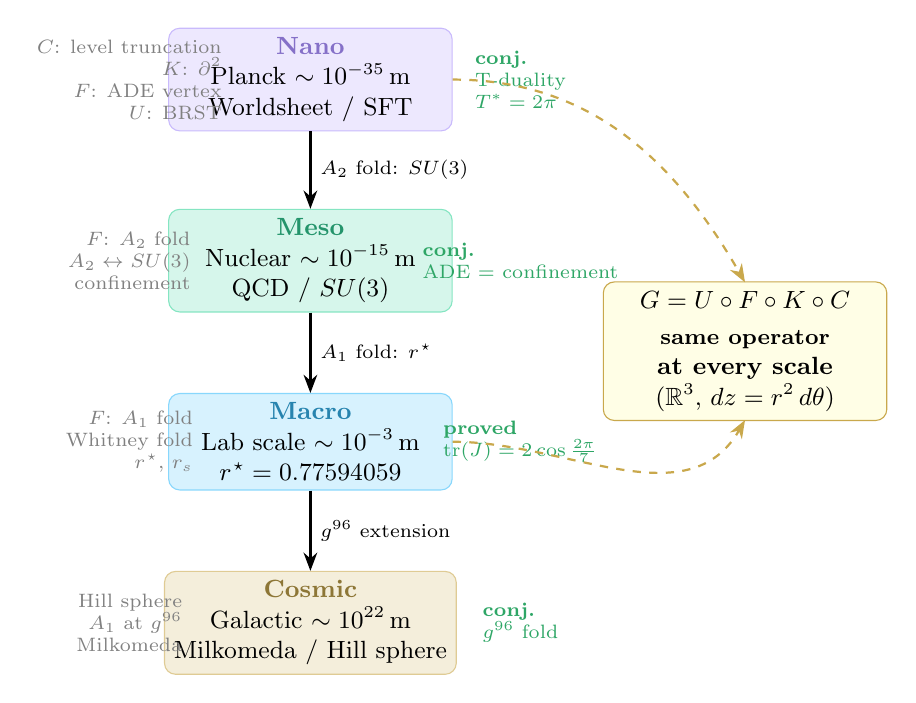
\begin{tikzpicture}[
  scale=0.92,
  box/.style={rounded corners=4pt,draw,align=center,font=\small,
              minimum width=3.6cm,minimum height=1.1cm},
  arr/.style={-Stealth,thick}
]
  % Nano box
  \node[box,fill=nano!20,draw=nano!60] (nano) at (0,6)
    {\textcolor{nano!80!black}{\bfseries Nano}\\
     Planck $\sim10^{-35}$\,m\\
     Worldsheet / SFT};

  % Meso box
  \node[box,fill=meso!20,draw=meso!60] (meso) at (0,3.5)
    {\textcolor{meso!70!black}{\bfseries Meso}\\
     Nuclear $\sim10^{-15}$\,m\\
     QCD / $SU(3)$};

  % Macro box
  \node[box,fill=macroC!20,draw=macroC!60] (macro) at (0,1)
    {\textcolor{macroC!70!black}{\bfseries Macro}\\
     Lab scale $\sim10^{-3}$\,m\\
     $\rstar=0.77594059$};

  % Cosmic box
  \node[box,fill=goldC!20,draw=goldC!60] (cosmic) at (0,-1.5)
    {\textcolor{goldC!70!black}{\bfseries Cosmic}\\
     Galactic $\sim10^{22}$\,m\\
     Milkomeda / Hill sphere};

  % Arrows
  \draw[arr] (nano) -- (meso)
    node[midway,right,font=\scriptsize] {$A_2$ fold: $SU(3)$};
  \draw[arr] (meso) -- (macro)
    node[midway,right,font=\scriptsize] {$A_1$ fold: $\rstar$};
  \draw[arr] (macro) -- (cosmic)
    node[midway,right,font=\scriptsize] {$g^{96}$ extension};

  % Left column: operator at each scale
  \node[align=right,font=\scriptsize,gray] at (-2.5,6)
    {$C$: level truncation\\$K$: $\partial^2$\\$F$: ADE vertex\\$U$: BRST};
  \node[align=right,font=\scriptsize,gray] at (-2.5,3.5)
    {$F$: $A_2$ fold\\$A_2\leftrightarrow SU(3)$\\confinement};
  \node[align=right,font=\scriptsize,gray] at (-2.5,1.0)
    {$F$: $A_1$ fold\\Whitney fold\\$\rstar$, $r_s$};
  \node[align=right,font=\scriptsize,gray] at (-2.5,-1.5)
    {Hill sphere\\$A_1$ at $g^{96}$\\Milkomeda};

  % Right column: proved/conj
  \node[align=left,font=\scriptsize,provedC] at (2.9,6)
    {{\bfseries conj.}\\T-duality\\$T^*=2\pi$};
  \node[align=left,font=\scriptsize,provedC] at (2.9,3.5)
    {{\bfseries conj.}\\ADE = confinement};
  \node[align=left,font=\scriptsize,provedC] at (2.9,1.0)
    {{\bfseries proved}\\$\mathrm{tr}(J)=2\cos\tfrac{2\pi}{7}$};
  \node[align=left,font=\scriptsize,provedC] at (2.9,-1.5)
    {{\bfseries conj.}\\$g^{96}$ fold};

  % Common element
  \node[box,fill=yellow!10,draw=goldC,font=\small\bfseries,
        minimum width=3.6cm] at (6,2.25)
    {$G=U\circ F\circ K\circ C$\\[2pt]
     \footnotesize same operator\\at every scale\\
     $(\mathbb{R}^3,\,dz=r^2\,d\theta)$};
  \draw[arr,dashed,goldC] (nano) to[out=0,in=120] (6,3.2);
  \draw[arr,dashed,goldC] (macro) to[out=0,in=240] (6,1.3);
\end{tikzpicture}
\caption{The dm$^3$ operator chain $G=U\circ F\circ K\circ C$ at four scales.
Left column: operator identifications at each scale.
Right column: proved (green) vs.\ conjectured.
The same contact manifold $(\mathbb{R}^3,\,dz=r^2\,d\theta)$ underlies every
level; the scale changes, the geometry does not.}
\label{fig:scales}
\end{figure}

% ─────────────────────────────────────────────────────────────────────────────
\section{The g-Series: Renormalization Group Ladder}
\label{sec:gseries}
% ─────────────────────────────────────────────────────────────────────────────

The $g$-series $g^0\to g^{64}$ is the renormalization-group (RG) scale ladder
connecting the Planck scale to the laboratory scale.

\begin{definition}[g-series]
The \emph{g-series} is the sequence of coupling vectors $\{g_i^{(n)}\}_{i\geq0}$
evolving under the RG transformation $\mathcal{R}_b$:
\[
  \{g_i^{(n+1)}\} = \mathcal{R}_b(\{g_i^{(n)}\}).
\]
A \emph{fixed point} satisfies $\mathcal{R}_b(G)=G$; the dm$^3$ operator chain
$G=U\circ F\circ K\circ C$ is conjectured to be such a fixed point, matching
the scale invariance implied by the contact condition $dz=r^2\,d\theta$.
\end{definition}

Key levels (see also Table~\ref{tab:gseries}):
\begin{itemize}[leftmargin=1.4em]
  \item \textbf{g$^6$ (seed)} — minimum viable seed; the cajueiro point.
    A system at g$^6$ has its first stable basin; it can branch to a new g$^6$
    after overshoot + resistance + lock. This cycle — \emph{seed → overshoot →
    resistance → new lock point → branch → new seed} — is the Cajueiro cycle,
    scale-invariant from a cashew tree ($\sim10^0$\,m) to a nebula ($\sim10^{16}$\,m).
  \item \textbf{g$^{64}$ (saturated)} — the laboratory Whitney $A_1$ fold:
    $\rstar=0.77594059$.
  \item \textbf{g$^{96}$} — galactic scale; Milkomeda as two overlapping
    g$^{96}$ limit-cycle basins.
  \item \textbf{g$^{64}\to$matrix} — at saturation the scalar series is
    conjectured to expand to $G_{\mathrm{matrix}}=[g_{ij}]$ where each entry
    is a full g$^0\to$g$^{64}$ cycle (Open Problem~\ref{op:matrix}).
\end{itemize}

\begin{table}[h]
\centering
\caption{The g-series scale ladder.}
\label{tab:gseries}
\begin{tabular}{@{}llll@{}}
\toprule
\textbf{Level} & \textbf{Scale (m)} & \textbf{Physics} & \textbf{Status}\\
\midrule
$g^0$--$g^4$ & $10^{-35}$--$10^{-31}$ & Planck / worldsheet & Conj.\\
$g^6$ (seed) & — & Minimum viable seed; first stable basin & Framework\\
$g^{16}$--$g^{32}$ & $10^{-18}$--$10^{-12}$ & QCD / $SU(3)$ $A_2$ fold & Conj.\\
$g^{32}$--$g^{48}$ & $10^{-12}$--$10^{-6}$ & Atomic / molecular & Conj.\\
$g^{64}$ (sat.) & $10^{-3}$--$10^1$ & $\rstar=0.77594059$; helical attractor & \textbf{Proved}\\
$g^{96}$ & $10^{9}$--$10^{22}$ & Hill sphere; Milkomeda & Conj.\\
$g^{64}\to$matrix & boundary & Quantum gravity re-enters & \textbf{Open}\\
\bottomrule
\end{tabular}
\end{table}

\begin{openproblem}[g$^{64}$ matrix extension]\label{op:matrix}
At saturation, the scalar g-series expands to a matrix
$G_{\mathrm{matrix}}=[g_{ij}]$
where each entry $g_{ij}$ is a full g$^0\to$g$^{64}$ scalar cycle.
This is structurally analogous to the BFSS matrix model~\cite{BFSS1997},
where quantum gravity emerges from D0-brane matrix quantum mechanics at the
Planck scale.
\end{openproblem}

% ─────────────────────────────────────────────────────────────────────────────
\section{Cosmic Scale: g$^{96}$ and Milkomeda}
\label{sec:milkomeda}
% ─────────────────────────────────────────────────────────────────────────────

The contact condition $dz=r^2\,d\theta$ is scale-free.
Keplerian orbits are contact-geometric: the angular-momentum first integral is
exactly $\alpha=0$ in an appropriate coordinate system.

\begin{conjecture}[Hill sphere as g$^{96}$ Whitney fold]
The Hill sphere — the boundary of a body's gravitational sphere of influence — is
a Whitney $A_1$ fold of the asymptotic orbital map at the g$^{96}$ level,
structurally identical to the laboratory fold at $\rstar$ but scaled by $\sim10^{25}$.
\end{conjecture}

The Milky Way--Andromeda merger (Milkomeda; expected $\sim4.5\times10^9$\,yr,
van der Marel et al.~\cite{vanderMarel2012}) is, in this framework:
two galactic-scale g$^{96}$ limit cycles whose outer basins of attraction overlap.
The merger is the fold event where the two attractors begin to coalesce.

\medskip\noindent\textbf{The Cajueiro Cycle.}
The g$^6\to$g$^{64}$ dynamics follow a universal cycle: a seed at g$^6$ overshoots
its equilibrium, encounters resistance, locks to a new stable band, branches, and
each branch seeds a new g$^6$.
The same pattern appears in:
cashew trees (Cajueiro; $\sim1$\,m), mycelium networks ($\sim10^{-3}$\,m),
geological fold mountains ($\sim10^4$\,m), nebular star formation ($\sim10^{16}$\,m).
\emph{Same geometry — different substrate.}

% ─────────────────────────────────────────────────────────────────────────────
\section{Bidirectionality and the Arrow of Time}
\label{sec:bidir}
% ─────────────────────────────────────────────────────────────────────────────

The ODE~\eqref{eq:r}--\eqref{eq:z} is time-reversible ($t\to-t$ maps attractor to
repeller and $\eps=+2$ to $\eps=-2$).
Gravity, magnetism, and centrifugal force are all time-reversible forces; time is
not.

In the dm$^3$ framework the operator $U$ (gradient descent) selects the stable branch
and thereby breaks the $t\to-t$ symmetry, introducing a preferred direction — the
thermodynamic arrow of time.
The duality $\eps=+2$ (attractive outer basin: matter) $\leftrightarrow$ $\eps=-2$
(repulsive outer basin: dual/antimatter) is the mathematical expression of the
time-reversal symmetry.
The ALPHA Collaboration~\cite{ALPHA2023} confirmed that antimatter falls
\emph{downward} (attracted by gravity), consistent with the $\eps=+2$ channel
dominating the observable universe.

% ─────────────────────────────────────────────────────────────────────────────
\section{Open Problems}
\label{sec:open}
% ─────────────────────────────────────────────────────────────────────────────

\begin{openproblem}[Closed-form $\rstar$]
Find an algebraic expression for $\rstar=0.77594059$.
The value is certified numerically; an exact form is unknown.
Lean~4 mechanisation in progress (AXLE,
\href{https://github.com/TOTOGT/AXLE}{\texttt{github.com/TOTOGT/AXLE}}).
\end{openproblem}

\begin{openproblem}[Sasakian QCD vacuum (F.5)]
Show that the contact manifold arising from the QCD vacuum geometry is
Sasakian-Einstein, connecting dm$^3$ to the
$\mathrm{AdS}_5\times SE_5$ family in AdS/CFT.
\end{openproblem}

\begin{openproblem}[g$^{64}$ matrix extension]
See Problem~\ref{op:matrix}.
\end{openproblem}

\begin{openproblem}[Galactic fold radius]
Derive the g$^{96}$ analog of $\rstar$ for galactic-scale attractors (Hill sphere
and Milkomeda).
\end{openproblem}

% ─────────────────────────────────────────────────────────────────────────────
\section{Empirical Grounding}
\label{sec:empirical}
% ─────────────────────────────────────────────────────────────────────────────

The contact geometry results stand independently of the string mathematical
framework (not a physical theory — no confirmed experimental predictions).
Every experimental claim is anchored in peer-reviewed measurement:

\begin{itemize}[leftmargin=1.4em]
\item $\rstar=0.77594059$ — certified numerically~\cite{certify};
  reproducible in under 2\,min.
\item Atom trap stable radius — Nobel lectures, Chu, Cohen-Tannoudji,
  Phillips 1997~\cite{Nobel1997}.
\item Antimatter gravity — ALPHA Collaboration, \textit{Nature} 615, 591--595
  (2023)~\cite{ALPHA2023}.
\item ADE gauge groups — McKay correspondence theorem~\cite{McKay1980}.
\item T-duality — Buscher (1987), standard result~\cite{Buscher1987}.
\item Sasakian geometry — Sparks (2011)~\cite{Sparks2011}.
\item Milkomeda merger timescale — van der Marel et al.\ (2012)~\cite{vanderMarel2012}.
\end{itemize}

% ─────────────────────────────────────────────────────────────────────────────
% REFERENCES
% ─────────────────────────────────────────────────────────────────────────────
\begin{thebibliography}{99}

\bibitem{Grossi2026togt}
P.N.~Grossi,
\textit{Contact-Geometric Theory of Generative Transitions: Mathematical Foundations,
Contact Realization, Seven Proofs of the Tribonacci Constant, and Applications to
Nuclear Matter},
\href{https://doi.org/10.5281/zenodo.20682934}{doi:10.5281/zenodo.20682934} (2026).

\bibitem{certify}
P.N.~Grossi, \texttt{certify\_rstar.py}, Verified at
\href{https://totogt.github.io/3M/law3m.html}{\texttt{totogt.github.io/3M/law3m.html}};
code: \href{https://github.com/TOTOGT/3M}{\texttt{github.com/TOTOGT/3M}} (2026).

\bibitem{Roy1975}
S.~Roy, ``Al-Biruni and Hindu Speculations on Gravitation,''
\textit{Indian Journal of History of Science} \textbf{10}(2), 218--223 (1975).

\bibitem{McKay1980}
J.~McKay, ``Graphs, singularities, and finite groups,''
\textit{Proc.\ Symp.\ Pure Math.} \textbf{37}, 183--186 (1980).

\bibitem{Buscher1987}
T.H.~Buscher, ``A symmetry of the string background field equations,''
\textit{Phys.\ Lett.\ B} \textbf{194}, 59--62 (1987).

\bibitem{Witten1986}
E.~Witten, ``Non-commutative geometry and string field theory,''
\textit{Nucl.\ Phys.\ B} \textbf{268}, 253--294 (1986).

\bibitem{Zwiebach1993}
B.~Zwiebach, ``Closed string field theory: quantum action and the
B-V master equation,'' \textit{Nucl.\ Phys.\ B} \textbf{390}, 33--152 (1993).

\bibitem{Sparks2011}
J.~Sparks, ``Sasaki-Einstein manifolds,''
\textit{Surveys in Differential Geometry} \textbf{16}, 265--324 (2011).

\bibitem{Blair2010}
D.E.~Blair, \textit{Riemannian Geometry of Contact and Symplectic Manifolds},
2nd ed., Birkhäuser (2010).

\bibitem{Washington1997}
L.C.~Washington, \textit{Introduction to Cyclotomic Fields},
2nd ed., Springer GTM 83 (1997).

\bibitem{Perko2001}
L.~Perko, \textit{Differential Equations and Dynamical Systems},
3rd ed., Springer TAM 7 (2001).

\bibitem{Polchinski1998}
J.~Polchinski, \textit{String Theory}, Vols.~I--II,
Cambridge University Press (1998).

\bibitem{BFSS1997}
T.~Banks, W.~Fischler, S.H.~Shuker, L.~Susskind,
``M theory as a matrix model: a conjecture,''
\textit{Phys.\ Rev.\ D} \textbf{55}, 5112--5128 (1997).

\bibitem{ALPHA2023}
ALPHA Collaboration, ``Observation of the effect of gravity on the motion of
antimatter,'' \textit{Nature} \textbf{615}, 591--595 (2023).

\bibitem{Nobel1997}
S.~Chu, C.~Cohen-Tannoudji, W.D.~Phillips,
Nobel Lectures in Physics 1997,
\textit{Rev.\ Mod.\ Phys.} \textbf{70}, 685--741 (1998).

\bibitem{vanderMarel2012}
R.P.~van der Marel et al.,
``The M31 Velocity Vector. III. Future Milky Way--M31--M33 Orbital Evolution,
Merging, and Fate of the Sun,''
\textit{Astrophys.\ J.} \textbf{753}, 9 (2012).

\end{thebibliography}

\vspace{.8em}
\noindent\rule{\linewidth}{0.4pt}\\[.3em]
{\small\textit{Principia Orthogona Series, ISBN 979-8-9954416-6-3.
ORCID: 0009-0000-6496-2186. CC BY 4.0.
Lean~4 mechanisation: \texttt{github.com/TOTOGT/AXLE}.}}

\end{document}
